
%(BEGIN_QUESTION)
% Copyright 2006, Tony R. Kuphaldt, released under the Creative Commons Attribution License (v 1.0)
% This means you may do almost anything with this work of mine, so long as you give me proper credit

En ventil er plassert på dampkjelens vanntrommel (noen ganger kalt ``mud''-trommelen), med formål å ``blåse ned'' kjelanlegget for å fjerne sedimenter og overskudd av mineralinnhold fra det ellers ultrarene vannet:

$$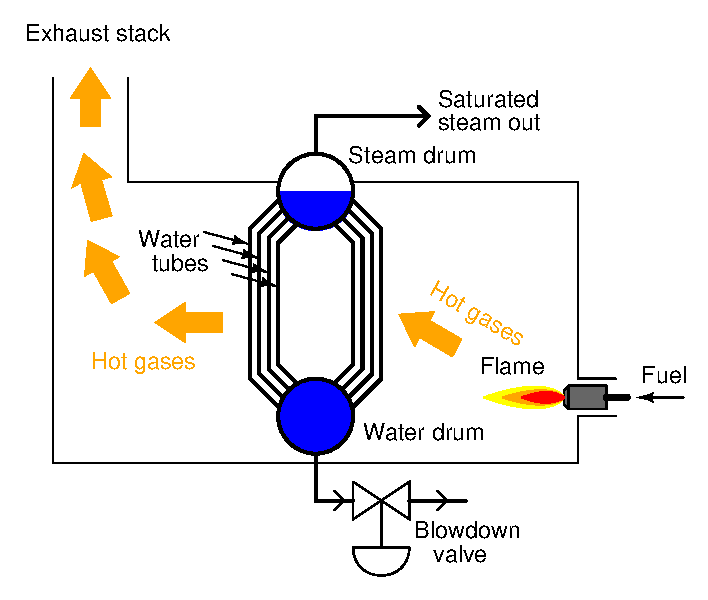
\includegraphics[width=15.5cm]{i01421x01.eps}$$

Ingeniøren som spesifiserte denne ventilen var relativt uerfaren, og det vises i ventilens ytelse. Selv om ventilens C$_{v}$ er korrekt dimensjonert for trykkfallet over den og tettheten til det varme vannet som strømmer gjennom den, viser det seg at ventilen slipper gjennom {\it mye} mindre vann enn forventet. Når den står fullt åpen, slipper blowdown-ventilen bare ut en liten del av den tiltenkte vannstrømmen, selv når nedstrømssiden er ventilert til atmosfæren, og hele kjelens trykkfall ligger over ventilen.

Hva er feil her? Hva hindrer blowdown-ventilen i å slippe gjennom nok vann når den er helt åpen?
 
\underbar{file i01421}
%(END_QUESTION)





%(BEGIN_ANSWER)

Svaret på dette spørsmålet (nei, jeg kommer ikke til å gi det bort direkte!) henger sammen med fysikken i oppvarmet vann under trykk. Hva skjer med en trykksatt væske når den slippes ut til atmosfæren, dersom væsketemperaturen ligger godt over kokepunktet ved atmosfærisk trykk?
 
%(END_ANSWER)





%(BEGIN_NOTES)

Når det varme kjelvannet går inn i ventilen, møter det et kraftig trykkfall og flasher over til damp. Den raske ekspansjonen fra vann til damp gir kvelning, som sterkt begrenser strømningen gjennom ventilen.

Ingeniørens feil i dimensjoneringen var å ignorere faseovergangen fra vann til damp ved trykkfall. Enten må ventilen dimensjoneres større, eller så må nedstrømstrykket ($P_2$) økes, for å eliminere dette problemet.

%INDEX% Final Control Elements, valve: choked flow
%INDEX% Final Control Elements, valve: sizing
%INDEX% Process: steam boiler blowdown

%(END_NOTES)

